\documentclass[11pt]{article}
\usepackage{amsmath, amsfonts, amsthm, amssymb}  % Some math symbols
\usepackage{lmodern}  % A modern version of LaTeX's famous default font. 
\usepackage{microtype}
\usepackage{fullpage}

\usepackage[x11names, rgb]{xcolor}
\usepackage{graphicx}
\usepackage{tikz}
\usetikzlibrary{decorations,arrows,shapes,automata,positioning}
\tikzset{
->, % makes the edges directed
% >=stealth’, % makes the arrow heads bold
node distance=1cm, % specifies the minimum distance between two nodes. Change if necessary.
every state/.style={thick, fill=gray!10}, % sets the properties for each ’state’ node
initial text=$ $, % sets the text that appears on the start arrow
auto
}

\usepackage{etoolbox}
\usepackage{enumerate}
\usepackage{listings}

\setlength{\parindent}{0pt}
\setlength{\parskip}{5pt plus 1pt}

\newcommand{\nopagenumbers}{
    \pagestyle{empty}
}

\def\indented#1{\list{}{}\item[]}
\let\indented=\endlist

\providetoggle{questionnumbers}
\settoggle{questionnumbers}{true}
\newcommand{\noquestionnumbers}{
    \settoggle{questionnumbers}{false}
}

\newcounter{questionCounter}
\newenvironment{question}[2][\arabic{questionCounter}]{%
    \addtocounter{questionCounter}{1}%
    \setcounter{partCounter}{0}%
    \vspace{.25in} \hrule \vspace{0.4em}%
        \noindent{\bf \iftoggle{questionnumbers}{#1: }{}#2}%
    \vspace{0.8em} \hrule \vspace{.10in}%
}{$ $\newpage}

\newcounter{partCounter}[questionCounter]
\renewenvironment{part}[1][\alph{partCounter}]{%
    \addtocounter{partCounter}{1}%
    \vspace{.10in}%
    \begin{indented}%
       {\bf (#1)} %
}{\end{indented}}

\def\show#1{\ifdefempty{#1}{}{#1\\}}




%%%%%%%%%%%%%%%%% Identifying Information %%%%%%%%%%%%%%%
%%		 		For 301, we'd rather you DIDN'T tell us who you are   		%%
%%				in your homework so that we're not biased when we     		%%
%% 				grade. So, even if you fill this information in, it   			%%
%% 				will not show up in the document unless you uncomment 		%%
%%				 \show\myname and \show\myemail below                  		%%
%%%%%%%%%%%%%%%%%%%%%%%%%%%%%%%%%%%%%%%%%%%
\newcommand{\myhwname}{Homework 2}
\newcommand{\myname}{Anon}
\newcommand{\myemail}{anon@uic.edu}
%%%%%%%%%%%%%%%%%%%%%%%%%%%%%%%%%%%%%%%%%%%%%%%%%%%%%%%%%%%
\newcommand{\header}{%
\begin{center}
    {\Large \show\myhwname}
    % \show\myname
    % \show\myemail
    \today
\end{center}}
%%%%%%%%%%%%%%%%%%% Document Options %%%%%%%%%%%%%%%%%%%%%%
% \noquestionnumbers
\nopagenumbers
%%%%%%%%%%%%%%%%%%%%%%%%%%%%%%%%%%%%%%%%%%%%%%%%%%%%%%%%%%%

\begin{document}
\header

\begin{question}{Regular Construction}
    \begin{part}
        $((a \cup b)^* bc(a \cup b)^* bc(a \cup b)^* bc)^* (a \cup b)^*$
    \end{part}

    \begin{part}
        
\begin{center}
    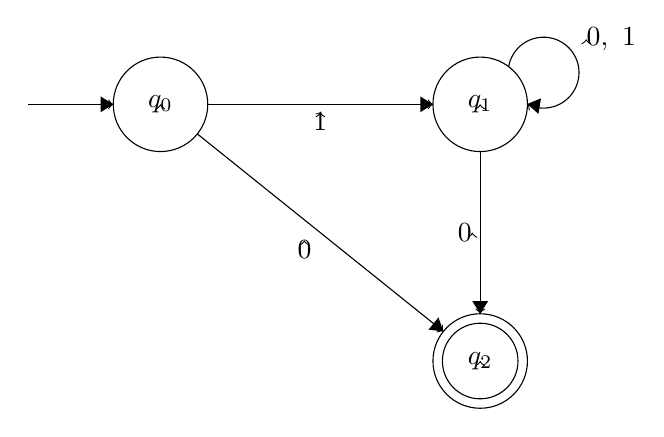
\begin{tikzpicture}[scale=0.2]
    \tikzstyle{every node}+=[inner sep=0pt]
    \draw [black] (23.4,-21) circle (3);
    \draw (23.4,-21) node {$q_0$};
    \draw [black] (43.7,-21) circle (3);
    \draw (43.7,-21) node {$q_1$};
    \draw [black] (43.7,-37.3) circle (3);
    \draw (43.7,-37.3) node {$q_2$};
    \draw [black] (43.7,-37.3) circle (2.4);
    \draw [black] (26.4,-21) -- (40.7,-21);
    \fill [black] (40.7,-21) -- (39.9,-20.5) -- (39.9,-21.5);
    \draw (33.55,-21.5) node [below] {$1$};
    \draw [black] (45.505,-18.619) arc (170.56505:-117.43495:2.25);
    \draw (50.43,-16.87) node [right] {$0,\mbox{ }1$};
    \fill [black] (46.69,-20.98) -- (47.4,-21.61) -- (47.56,-20.62);
    \draw [black] (43.7,-24) -- (43.7,-34.3);
    \fill [black] (43.7,-34.3) -- (44.2,-33.5) -- (43.2,-33.5);
    \draw (43.2,-29.15) node [left] {$0$};
    \draw [black] (25.74,-22.88) -- (41.36,-35.42);
    \fill [black] (41.36,-35.42) -- (41.05,-34.53) -- (40.42,-35.31);
    \draw (32.54,-29.64) node [below] {$0$};
    \draw [black] (15,-21) -- (20.4,-21);
    \fill [black] (20.4,-21) -- (19.6,-20.5) -- (19.6,-21.5);
    \end{tikzpicture}
    \end{center}
    
    \end{part}
\end{question}

\begin{question}{NFA to RegEx Conversion}
    
\begin{center}
    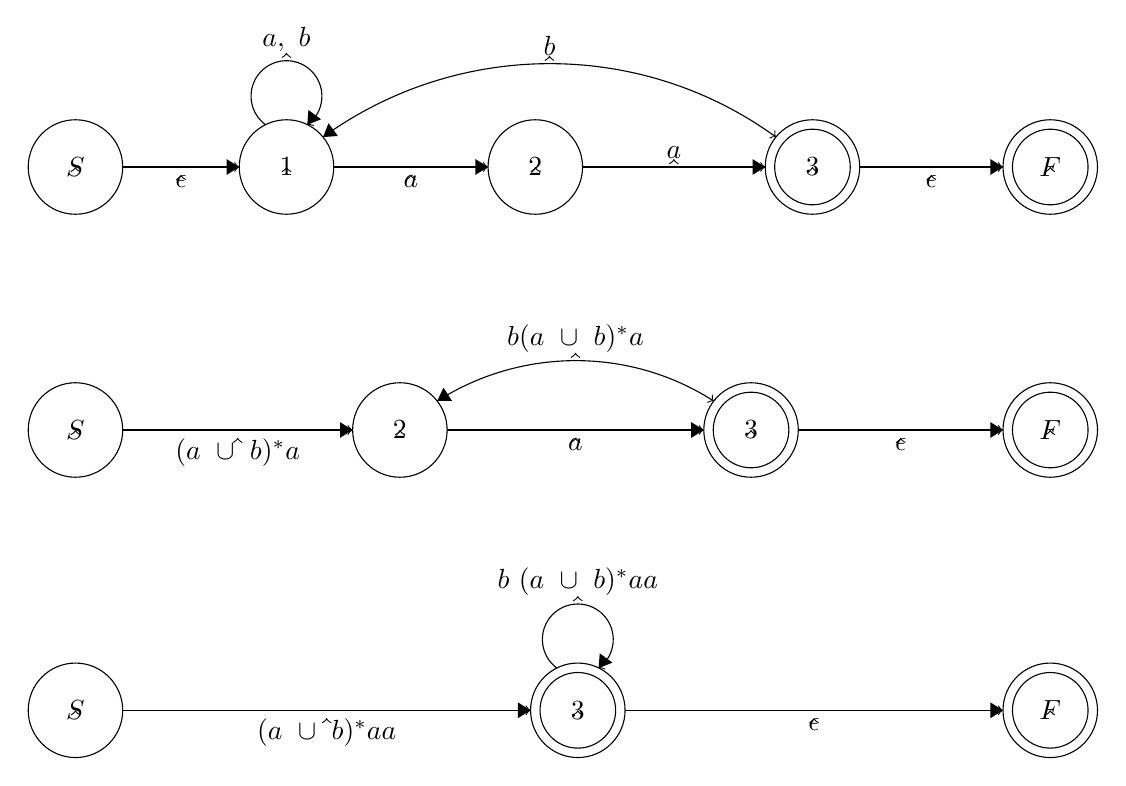
\begin{tikzpicture}[scale=0.2]
    \tikzstyle{every node}+=[inner sep=0pt]
    \draw [black] (19.7,-14.6) circle (3);
    \draw (19.7,-14.6) node {$1$};
    \draw [black] (35.5,-14.6) circle (3);
    \draw (35.5,-14.6) node {$2$};
    \draw [black] (53.1,-14.6) circle (3);
    \draw (53.1,-14.6) node {$3$};
    \draw [black] (53.1,-14.6) circle (2.4);
    \draw [black] (68.2,-14.6) circle (3);
    \draw (68.2,-14.6) node {$F$};
    \draw [black] (68.2,-14.6) circle (2.4);
    \draw [black] (6.3,-14.6) circle (3);
    \draw (6.3,-14.6) node {$S$};
    \draw [black] (6.3,-31.3) circle (3);
    \draw (6.3,-31.3) node {$S$};
    \draw [black] (26.9,-31.3) circle (3);
    \draw (26.9,-31.3) node {$2$};
    \draw [black] (49.2,-31.3) circle (3);
    \draw (49.2,-31.3) node {$3$};
    \draw [black] (49.2,-31.3) circle (2.4);
    \draw [black] (68.2,-31.3) circle (3);
    \draw (68.2,-31.3) node {$F$};
    \draw [black] (68.2,-31.3) circle (2.4);
    \draw [black] (6.3,-49.1) circle (3);
    \draw (6.3,-49.1) node {$S$};
    \draw [black] (38.2,-49.1) circle (3);
    \draw (38.2,-49.1) node {$3$};
    \draw [black] (38.2,-49.1) circle (2.4);
    \draw [black] (68.2,-49.1) circle (3);
    \draw (68.2,-49.1) node {$F$};
    \draw [black] (68.2,-49.1) circle (2.4);
    \draw [black] (9.3,-14.6) -- (16.7,-14.6);
    \fill [black] (16.7,-14.6) -- (15.9,-14.1) -- (15.9,-15.1);
    \draw (13,-15.1) node [below] {$\epsilon$};
    \draw [black] (18.377,-11.92) arc (234:-54:2.25);
    \draw (19.7,-7.35) node [above] {$a,\mbox{ }b$};
    \fill [black] (21.02,-11.92) -- (21.9,-11.57) -- (21.09,-10.98);
    \draw [black] (22.7,-14.6) -- (32.5,-14.6);
    \fill [black] (32.5,-14.6) -- (31.7,-14.1) -- (31.7,-15.1);
    \draw (27.6,-15.1) node [below] {$a$};
    \draw [black] (38.5,-14.6) -- (50.1,-14.6);
    \fill [black] (50.1,-14.6) -- (49.3,-14.1) -- (49.3,-15.1);
    \draw (44.3,-14.1) node [above] {$a$};
    \draw [black] (56.1,-14.6) -- (65.2,-14.6);
    \fill [black] (65.2,-14.6) -- (64.4,-14.1) -- (64.4,-15.1);
    \draw (60.65,-15.1) node [below] {$\epsilon$};
    \draw [black] (22.018,-12.698) arc (125.87477:54.12523:24.543);
    \fill [black] (22.02,-12.7) -- (22.96,-12.63) -- (22.37,-11.82);
    \draw (36.4,-7.54) node [above] {$b$};
    \draw [black] (9.3,-31.3) -- (23.9,-31.3);
    \fill [black] (23.9,-31.3) -- (23.1,-30.8) -- (23.1,-31.8);
    \draw (16.6,-31.8) node [below] {$(a\mbox{ }\cup\mbox{ }b)^*a$};
    \draw [black] (52.2,-31.3) -- (65.2,-31.3);
    \fill [black] (65.2,-31.3) -- (64.4,-30.8) -- (64.4,-31.8);
    \draw (58.7,-31.8) node [below] {$\epsilon$};
    \draw [black] (29.9,-31.3) -- (46.2,-31.3);
    \fill [black] (46.2,-31.3) -- (45.4,-30.8) -- (45.4,-31.8);
    \draw (38.05,-31.8) node [below] {$a$};
    \draw [black] (29.267,-29.464) arc (122.54445:57.45555:16.327);
    \fill [black] (29.27,-29.46) -- (30.21,-29.45) -- (29.67,-28.61);
    \draw (38.05,-26.4) node [above] {$b(a\mbox{ }\cup\mbox{ }b)^*a$};
    \draw [black] (9.3,-49.1) -- (35.2,-49.1);
    \fill [black] (35.2,-49.1) -- (34.4,-48.6) -- (34.4,-49.6);
    \draw (22.25,-49.6) node [below] {$(a\mbox{ }\cup\mbox{ }b)^*aa$};
    \draw [black] (41.2,-49.1) -- (65.2,-49.1);
    \fill [black] (65.2,-49.1) -- (64.4,-48.6) -- (64.4,-49.6);
    \draw (53.2,-49.6) node [below] {$\epsilon$};
    \draw [black] (36.877,-46.42) arc (234:-54:2.25);
    \draw (38.2,-41.85) node [above] {$b\mbox{ }(a\mbox{ }\cup\mbox{ }b)^*aa$};
    \fill [black] (39.52,-46.42) -- (40.4,-46.07) -- (39.59,-45.48);
    \end{tikzpicture}
    \end{center}
\begin{center}
    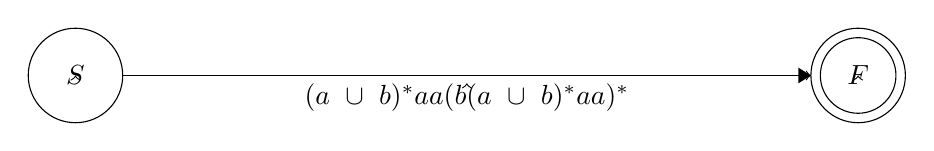
\begin{tikzpicture}[scale=0.2]
    \tikzstyle{every node}+=[inner sep=0pt]
    \draw [black] (18.8,-23.5) circle (3);
    \draw (18.8,-23.5) node {$S$};
    \draw [black] (68.5,-23.5) circle (3);
    \draw (68.5,-23.5) node {$F$};
    \draw [black] (68.5,-23.5) circle (2.4);
    \draw [black] (21.8,-23.5) -- (65.5,-23.5);
    \fill [black] (65.5,-23.5) -- (64.7,-23) -- (64.7,-24);
    \draw (43.65,-24) node [below] {$(a\mbox{ }\cup\mbox{ }b)^*aa(b(a\mbox{ }\cup\mbox{ }b)^*aa)^*$};
    \end{tikzpicture}
    \end{center}
    RegEx = $(a \cup b)^*aa(b(a \cup b)^*aa)^*$
\end{question}

\begin{question}{More than Regular}
    Suppose, for the sake of contradiction, that A is regular. Then by definition, there is a DFA M for which there is a pumping lumma, p. Let $s = 0^p1^{(p + 1)}$. By the pumping lumma, we can divide s into x, y, z where $|xy| \le p$ and $|y| \ge 1$. Then $y = 0^k$ represent the number of 0's for $0 < k \le p$. Pumping up gives us $xy^2z = 0^{(p + k)}1^{(p + 1)}.$ Since $k \ge 1$, then $p + k \ge p + 1$. Therefore, the number of 0's will be greater than or equal to the number of 1's Thus, there is a contradiction because $xy^2z \notin A$. Thus, A cannot be regular.
\end{question}
\end{document}
